%%%%%%%%%%%%%%%%%%%%%%%%%%%%%%%%%%%%%%%%%%%%%%%%%%%%%%
%if you install these packages on your machine, you can remove the relative path
%%%%%%%%%%%%%%%%%%%%%%%%%%%%%%%%%%%%%%%%%%%%%%%%%%%%%%
\documentclass[preprint,authoryear]{../../Stylesheets/elsarticle/elsarticle}

%%%%%%%%%%%%%%%%%%%%%%%%%%%%%%%%%%%%%%%%%%%%%%%%%%%%%%
% Include the packages (in IncludePackages.tex) and some new commands you may
% find useful (in NewCommands.tex). In SetupPackages.tex, additional set-up for
% packages that require this can be added.
%%%%%%%%%%%%%%%%%%%%%%%%%%%%%%%%%%%%%%%%%%%%%%%%%%%%%%
\usepackage{../../Stylesheets/DondersInstitute/customcommands}
\usepackage{fancyhdr}
\usepackage{amsmath}
\usepackage{amssymb}
\usepackage[pdftex]{hyperref}
\usepackage{subfigure}
\usepackage{natbib}
%%%%%%%%%%%%%%%%%%%%%
% Number sets
%%%%%%%%%%%%%%%%%%%%%
\newcommand{\reals}{\mathbb{R}}
\newcommand{\integers}{\mathbb{N}}


%%%%%%%%%%%%%%%%%%%%%
% \etalii
%%%%%%%%%%%%%%%%%%%%%
\newcommand{\etalii}[0]{\emph{et al. }}


%%%%%%%%%%%%%%%%%%%%%
% \diag
%%%%%%%%%%%%%%%%%%%%%
\newcommand{\diag}[0]{\text{diag}}

%%%%%%%%%%%%%%%%%%%%%
% \defeq
% ('is defined as' def equal sign)
%%%%%%%%%%%%%%%%%%%%%
\newcommand{\defeq}{\mathrel{\stackrel{\makebox[0pt]{\mbox{\normalfont\tiny def}}}{=}}}

%%%%%%%%%%%%%%%%%%%%%%%%%%%%%%%%%%%%
% This defines how the numbering works for of equations and figures
%%%%%%%%%%%%%%%%%%%%%%%%%%%%%%%%%%%%
\numberwithin{equation}{section}
\numberwithin{figure}{section}


%%%%%%%%%%%%%%%%%%%%%%%%%%%%%%%%%%%%
% This defines whether we always want to jump to a new page after a
% section (false) or stay on the same page if possible (true).
%%%%%%%%%%%%%%%%%%%%%%%%%%%%%%%%%%%%
\setboolean{savethetrees}{false}


%%%%%%%%%%%%%%%%%%%%%%%%%%%%%%%%%%%%
% This sets up the \autoref command, and defines how different types 
% things (equaitons, figures, sections, etc.) should be referred to. Use
% \autoref rather than \ref, cause if rocks!
%%%%%%%%%%%%%%%%%%%%%%%%%%%%%%%%%%%%
\def\chapterautorefname{Chapter}
\def\figureautorefname{Fig.}
\def\subfigureautorefname{Fig.}
\def\subfloatautorefname{Fig.}
\def\equationautorefname{Eq.}
\def\sectionautorefname{Sec.}
\def\subsectionautorefname{Sec.}
\def\subsubsectionautorefname{Sec.}


%%%%%%%%%%%%%%%%%%%%%%%%%%%%%%%%%%%%%%%%%%%%%%%%%%%%%%
% Define the graphics path (i.e. where you have all your pictures). If you want multiple
% folders with pictures, do: \graphicspath{{./Images/},{./MoreImages/}}
\graphicspath{{./Images/}}


%%%%%%%%%%%%%%%%%%%%%%%%%%%%%%%%%%%%%%%%%%%%%%%%%%%%%%
% Overwrite a boolean set earlier cause we like trees:
%%%%%%%%%%%%%%%%%%%%%%%%%%%%%%%%%%%%%%%%%%%%%%%%%%%%%%
\setboolean{savethetrees}{true}


%%%%%%%%%%%%%%%%%%%%%%%%%%%%%%%%%%%%%%%%%%%%%%%%%%%%%%
% BEGIN DOCUMENT 
%%%%%%%%%%%%%%%%%%%%%%%%%%%%%%%%%%%%%%%%%%%%%%%%%%%%%%
\begin{document} 



%%%%%%%%%%%%%%%%%%%%%%%%%%%%%%
% This starts the 'front matter', which everything preceding
% the actual contents of the paper.
%%%%%%%%%%%%%%%%%%%%%%%%%%%%%%
\begin{frontmatter}


%%%%%%%%%%%%%%%%%%%%%%%%%%%%%%
% Here we define things like the title, the authors, their
% contact details etcetera.
%%%%%%%%%%%%%%%%%%%%%%%%%%%%%% 
\journal{NeuromImage}
\title{On Elephants}
\author[DccnAddres]{Tim van Mourik}
\author[YorkAddress,SonyAddress]{Jelle van Mourik}

\address[DccnAddres]{Donders Institute for Brain, Cognition and Behaviour, Radboud University Nijmegen, 6525 EN Nijmegen, The Netherlands}
\address[YorkAddress]{The Department of Electronics, The University of York, Heslington, York, North Yorkshire, YO10 5DD}
\address[SonyAddress]{Sony Computer Entertainment Europe, 10-15 Great Marlborough St, London W1F 7HR, United Kingdom}


%%%%%%%%%%%%%%%%%%%%%%%%%%%%%%
% Add relevant key words here.
%%%%%%%%%%%%%%%%%%%%%%%%%%%%%%
\begin{keyword}
\begin{abstract}
This is a style sheet of a paper with highly sophisticated text, related to the scientific nature of pink elephants. Although pink elephants were recently thought to be extinct, this article proves that dodos never even existed. Therefore, since correlation does not imply causation, this statement is claimed to be false. The author cannot be held responsible for any damage this may cause to the trees in the rainforest of the Amazone.
\end{abstract}
Elephantology, Pink, Hippopotamus
\end{keyword}

\end{frontmatter}
%%%%%%%%%%%%%%%%%%%%%%%%%%%%%%



%%%%%%%%%%%%%%%%%%%%%%%%%%%%%%
% Here go all the chapters we want to include
%%%%%%%%%%%%%%%%%%%%%%%%%%%%%%
\begin{abstract}
This is a style sheet of a paper with highly sophisticated text, related to the scientific nature of pink elephants. Although pink elephants were recently thought to be extinct, this article proves that dodos never even existed. Therefore, since correlation does not imply causation, this statement is claimed to be false. The author cannot be held responsible for any damage this may cause to the trees in the rainforest of the Amazone.
\end{abstract}
\newpage
\section{Introduction}
\label{sec:Introduction}
For many years, the existence of pink elephants has been hypothesised. Flamingoes are pink, penguins are not pink, so there must be pink elephants as well.

Fig.~\ref{NotAPinkElephant} shows what a pink elephant does not look like:
\begin{figure}[h]
\begin{center}
	\subfigure[A grey elephant. Definitely not pink.]{\label{GreyElephant} 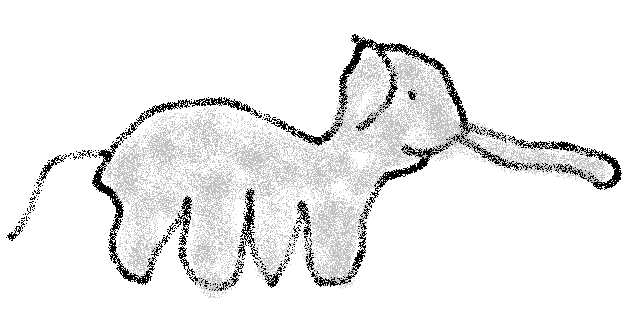
\includegraphics[width=0.33\textwidth]{GreyElephant} }
	\subfigure[A common misconception is that pinkuins are pink. This is not true and apart from that, they are not elephants either]{\label{Pinkuin} 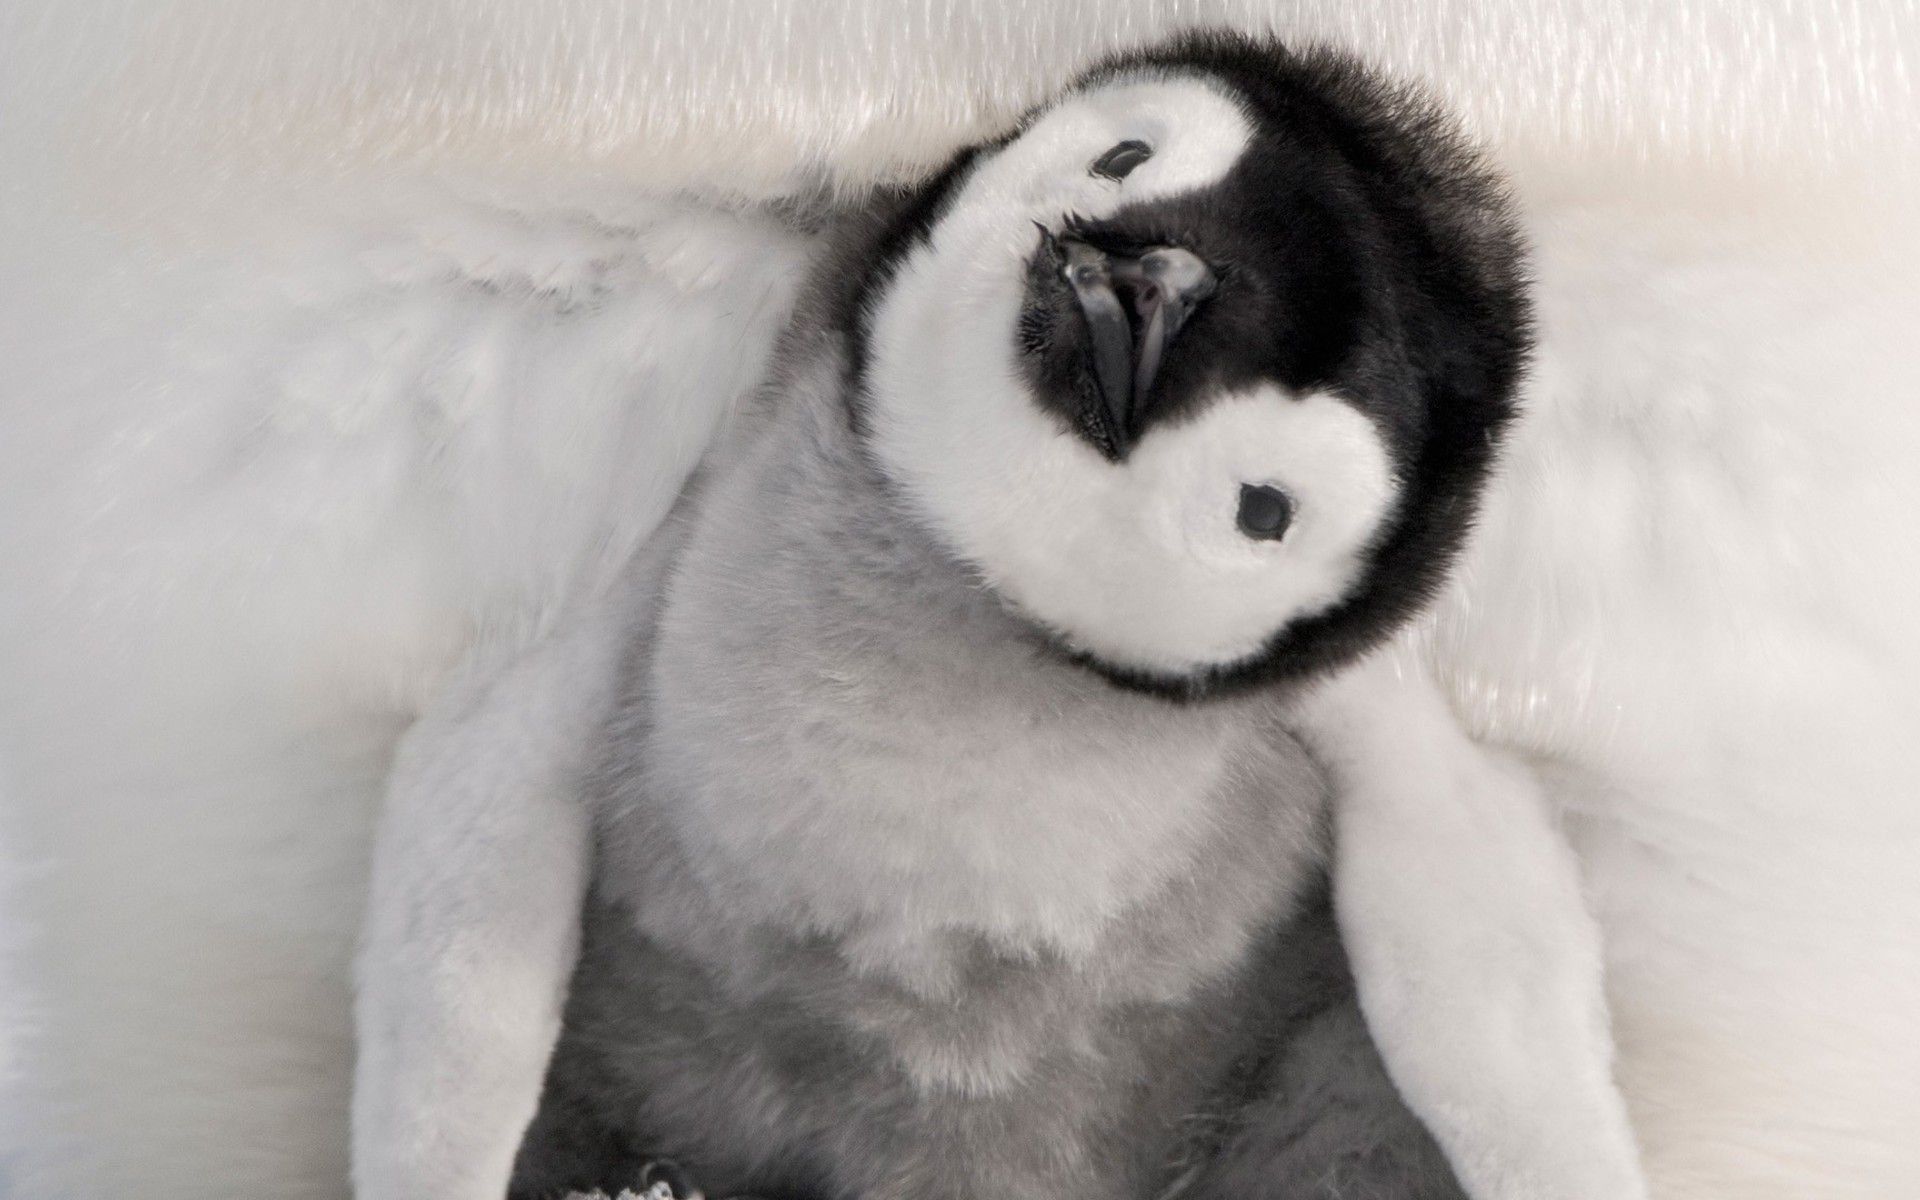
\includegraphics[width=0.33\textwidth]{Pinkuin} }
	\caption{non-pink non-elephants.}
	\label{NotAPinkElephant}
\end{center}
\end{figure} 

\savethetrees
\section{Methods}
\label{sec:Methods}

\subsection{Pink elephants}
Pink elephants are generally orange, but they can be blue instead. There are several different species:
\begin{itemize}
\item The \emph{Blue Pink Elephant}, recognisable by its green colour.
\item The \underline{Checkerboard Eared Pink Elephant}, which can be recognised by its ears in the shape of a chess board.
\item The \textbf{Happy Pink Elephant}, which loves dancing.
\end{itemize}
All of these species are extinct.

\subsection{Chickens}
Chickens are not elephants. Generalising this principle, we get
\begin{equation}
	P_{Chicken} = (p - a)(p - b)(p - c) ... (p - z)P_{Elephant},
	\label{eq:Equation1}
\end{equation}
where $P_{Chicken}$ stands for the population of cows in The Netherlands. Thus, equation \ref{eq:Equation1} does not have any implications for the population density of poisonous rubber duckies in Nigeria, since correlation does not imply causation. $\mathbf{QED}$

% Normally, LaTeX just jumps to a new page itself, of course. But if you want to manipulate its decisions, use this command:
\newpage 

\subsection{Hippopotamus}
It was proven by C. Rocodile \cite{Rocodile2014} that pink elephants have absolutely nothing to do with hippopotamuses. Figure \ref{fig:Elephant} is not a picture of a hippopotamus:
\begin{figure}[h]
	\centering
	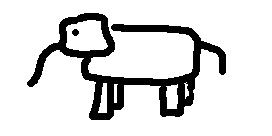
\includegraphics[width=150pt]{ElephantSimple}
	\caption{Not a hippo}
	\label{fig:Elephant}
\end{figure}

\subsubsection{Hippopotamidae and math}
Hippopotami amphibii luuuv complicated looking math equations. The following is an example of an equation that a hippo notoriously solved by taking the Fourier Transform twice\footnote{...and swallowed another banana....}, after which he retired:
\begin{equation}
	\sum_{\substack{ 1 < i \leq \infty \\ j \neq i}}  \frac{\partial}{\partial \xi} \oint \mathcal{A + B} 
			\begin{pmatrix} 1 & 2 & 3 \\  4 & 5 & 6 \end{pmatrix} = \left(	x \frac{e^{2 \pi i \omega}}{r^2}	\right)^2
\end{equation}

\savethetrees
\section{Results}
\label{sec:Results}
All in all, pink elephants can be quite the elephant in the room, as can be seen in Fig.~\ref{fig:ElephantInRoom}.
\begin{figure}[h]
	\centering
	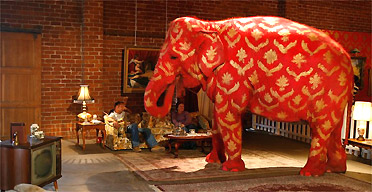
\includegraphics[width=150pt]{ElephantInRoom}
	\caption{The elephant in the room}
	\label{fig:ElephantInRoom}
\end{figure}

Pink elephants are widely revered throughout popular and impopular culture. Statues as well as look alikes of elephants have been erected, as shown in Fig.~\ref{ElephantsInCulture}

\begin{figure}[h]
\begin{center}
	\subfigure[Statue of elephant]{\label{Statue} 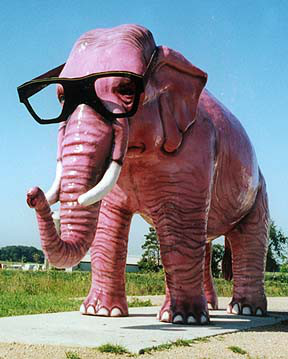
\includegraphics[width=0.33\textwidth]{Statue} }
	\subfigure[Elephant look alike]{\label{Tank} 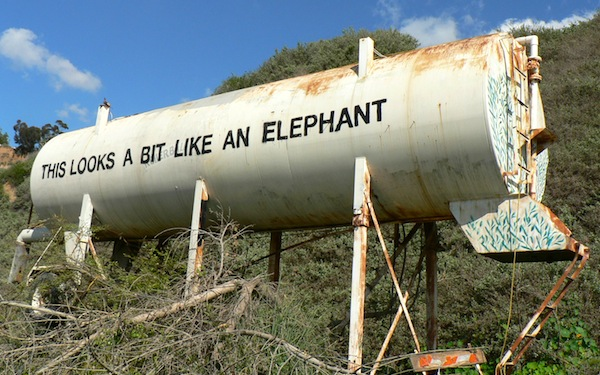
\includegraphics[width=0.33\textwidth]{NotAnElephant} }
	\caption{Elephants in popular and impopular culture.}
	\label{ElephantsInCulture}
\end{center}
\end{figure} 

\savethetrees
\section{Discussion}
\label{sec:Discussion}
In this paper we debunked the common myth that pink elephants are causing delirium tremens. As mentioned before, correlation does not imply causation and hence we hypothesise that delirium causes a sudden increase in pink elephants birth rates.
\begin{figure}[h]
	\centering
	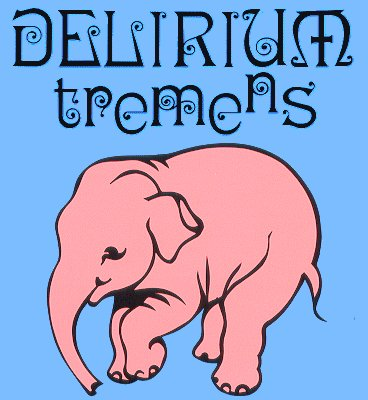
\includegraphics[width=150pt]{Delirium}
	\caption{Delirium elephans}
	\label{fig:ElephantTremens}
\end{figure}

\savethetrees
\section{Conclusion}
\label{sec:Conclusion}
This was the end of the hippo, and also of this tutorial about the intricacies of \LaTeX. Please use MS Word in the future, if the colour of the ribbons displeaseth thy eyes. 

And then there came an elephant with a long snout, who blew this story out.
\savethetrees
%%%%%%%%%%%%%%%%%%%%%%%%%%%%
\section{Acknowledgements}
\label{sec:Acknowledgements}
%%%%%%%%%%%%%%%%%%%%%%%%%%%%

Thanks go out to Jelle van Mourik, who was willing to share is ideas on \LaTeX-stylesheets and his extensive research on elephants and hippos. Furthermore, we would like to thank all people that have shared their thoughts on pink elephants with us.
\savethetrees

%%%%%%%%%%%%%%%%%%%%%%%%%%%%%%
% This defines the bibliography style (e.g. plain) , and 
% references the .bib file with all your references.
%%%%%%%%%%%%%%%%%%%%%%%%%%%%%%
\bibliographystyle{plain}
\bibliography{../../Bibliography/Bibliography}


%%%%%%%%%%%%%%%%%%%%%%%%%%%%%%
% Add some appendices if you like.
%%%%%%%%%%%%%%%%%%%%%%%%%%%%%%
\onecolumn
%\appendix
%\begin{appendices}

%\end{appendices}
%\newpage
%%\section*{Figures}


%%%%%%%%%%%%%%%%%%%%%
\end{document}
%%%%%%%%%%%%%%%%%%%%%




